\documentclass[10.5pt,scale=1.0,t,aspectratio=169,hyperref={pdfpagelabels=false}]{beamer}


\usepackage{lipsum}
\usepackage{color}
\usepackage{amsfonts}
\usepackage{amsmath,mathtools}
\usepackage{mathrsfs}
\usepackage{array}
\usepackage{algorithm}
\usepackage{hyperref}
\usepackage[spanish,es-nodecimaldot]{babel}
\usepackage[utf8]{inputenc}
\usepackage{graphicx}
\usepackage{multicol}
\usepackage{multirow}
\usepackage{enumitem}
\usepackage[document]{ragged2e}
\usepackage[absolute,overlay]{textpos}
\textblockorigin{0mm}{0mm} 
\usefonttheme[onlymath]{serif}
\usepackage{verbatim}
\usepackage{cite}
\usepackage{multicol}
\usepackage{siunitx}
\usepackage{mathtools}
\DeclarePairedDelimiter\ceil{\lceil}{\rceil}
\DeclarePairedDelimiter\floor{\lfloor}{\rfloor}




\newenvironment{conditions}[1][where:]
{#1 \begin{tabular}[t]{>{$}l<{$} @{${}={}$} l}}
	{\end{tabular}\\[\belowdisplayskip]}


\newcolumntype{L}{>{$}l<{$}} % math-mode version of "l" column type


\newcounter{saveenumi}
\newcommand{\seti}{\setcounter{saveenumi}{\value{enumi}}}
\newcommand{\conti}{\setcounter{enumi}{\value{saveenumi}}}

\setbeamertemplate{bibliography item}{\insertbiblabel}


\hypersetup{colorlinks=true,
	linkcolor=blue,
	linktoc=all,				
	citecolor=blue,
	urlcolor=red,
	pdftitle={ELECTRONICA DIGITAL},
	pdfauthor={Santiago Rúa Pérez},
	pdfcreator={Santiago Rúa Pérez}}


\definecolor{GreenDark}{rgb}{0.0, 0.60, 0.0}
\definecolor{RedDark}{rgb}{183, 0.0, 0.0}
\definecolor{BlueDark}{rgb}{0.0, 0.0, 167}
\definecolor{BlueLight}{rgb}{0.2, 0.451, 0.517}


\graphicspath{{imag/}}

\newcommand{\Ho}{$H_{0}$}
\newcommand{\Ha}{$H_{a}$}
\newcommand{\Nota}{{\bf Nota: }}
\newcolumntype{P}[1]{>{\centering\arraybackslash}p{#1}}
\newcolumntype{M}[1]{>{\centering\arraybackslash}m{#1}}

\newcommand{\less}{<}
\newcommand{\greater}{>}


\setlength{\parindent}{1em}
\setlength{\parskip}{.6em}
\renewcommand{\baselinestretch}{.9}

%%%%    C environment    ---------------- %%%%%%%%%%%%%%%.
\usepackage{listings}
\usepackage{xcolor}
\definecolor{mGreen}{rgb}{0,0.6,0}
\definecolor{mGray}{rgb}{0.5,0.5,0.5}
\definecolor{mPurple}{rgb}{0.58,0,0.82}
\definecolor{backgroundColour}{rgb}{0.95,0.95,0.92}

\lstdefinestyle{CStyle}{
	backgroundcolor=\color{backgroundColour},   
	commentstyle=\color{mGreen},
	keywordstyle=\color{magenta},
	numberstyle=\tiny\color{mGray},
	stringstyle=\color{mPurple},
	basicstyle=\scriptsize,
	breakatwhitespace=false,         
	breaklines=true,                 
	captionpos=b,                    
	keepspaces=true,                 
	numbers=left,                    
	numbersep=5pt,                  
	showspaces=false,                
	showstringspaces=false,
	showtabs=false,                  
	tabsize=2,
	language=C
}
%%--------------------------------------------------------------------------


\title{Electrónica Digital II}   
\author{Santiago Rúa Pérez, PhD.} 
\date{\today} 

\setlength{\TPHorizModule}{\textwidth}
\setlength{\TPVertModule}{\textwidth}

\newcommand{\btVFill}{\vskip0pt plus 1filll}


\setbeamertemplate{sidebar right}{}
\setbeamertemplate{footline}
{
	\leavevmode%
	\hbox{%
		\begin{beamercolorbox}[wd=.333333\paperwidth,ht=2.25ex,dp=1ex,center]{author in head/foot}%
			\usebeamerfont{author in head/foot}\insertshortauthor
		\end{beamercolorbox}%
		\begin{beamercolorbox}[wd=.333333\paperwidth,ht=2.25ex,dp=1ex,center]{title in head/foot}%
			\usebeamerfont{title in head/foot}\insertshorttitle
	\end{beamercolorbox}}%
	\vskip0pt%
}
\makeatother

\begin{document}
	%%%%%%%%%%%%%%%%%% FRAME %%%%%%%%%%%%%%%%%%%%%%%%%%
	\begin{frame}
		\titlepage
	\end{frame}
	%%%%%%%%%%%%%%%%% FRAME START %%%%%%%%%%%%%%%%%%%%%%%%%%
	\frame{
		%\frametitle{}
		\begin{center}
			\LARGE \textcolor{blue}{INTERFAZ ANÁLOGA}
		\end{center}
		
	}
	
	%%%%%%%%%%%%%%%%% FRAME %%%%%%%%%%%%%%%%%%%%%%%%%%

%%%%%%%%%%%%%%%%% FRAME %%%%%%%%%%%%%%%%%%%%%%%%%%
\begin{frame}
\frametitle{Objetivos}
\begin{itemize}
\item Entender el funcionamiento de una interfaz análoga en un sistema embebido. 
\item Entender el funcionamiento de un conversor SAR.
\item Comprender la configuración de registros para la lectura de un puerto convertidor. 
\end{itemize}
\end{frame}
%%%%%%%%%%%%%%%%% FRAME %%%%%%%%%%%%%%%%%%%%%%%%%%
\begin{frame}
	\frametitle{Porque es necesario?}
	\begin{itemize}
		\item Los sistemas embebidos a menudo requieren medir parámetros físicos.
		\item Usualmente estos parámetros físicos son continuos (análogos) y no se encuentran en forma digital las cuales pueden ser procesados por las computadores 
		\item Algunas de estas variables son:
		\begin{itemize}
			\item \textbf{Temperatura}: termómetros, controlador de motores en un carro, monitoreo en un reactor químico, seguridad en los microcontroladores. 
			\item \textbf{Luz o intensidad de luz}: cámara digital, receptor IR, monitor UV.
			\item \textbf{Posición angular}: medidor de viento o nudos. 
			\item \textbf{Presión}: monitores de la presión sanguínea, altímetro, controlador en carro, detector de tsunami. 
			\item \textbf{Aceleración}: estabilidad del vehículo, controles de video juegos. 
			\item \textbf{Otros}: controlador de touchscreen, EKG, EEG, etc. 
		\end{itemize}
	\end{itemize}
\end{frame}
%%%%%%%%%%%%%%%%% FRAME %%%%%%%%%%%%%%%%%%%%%%%%%%
\begin{frame}
	\frametitle{Panorama general - Ejemplo}
	\begin{figure}
		\centering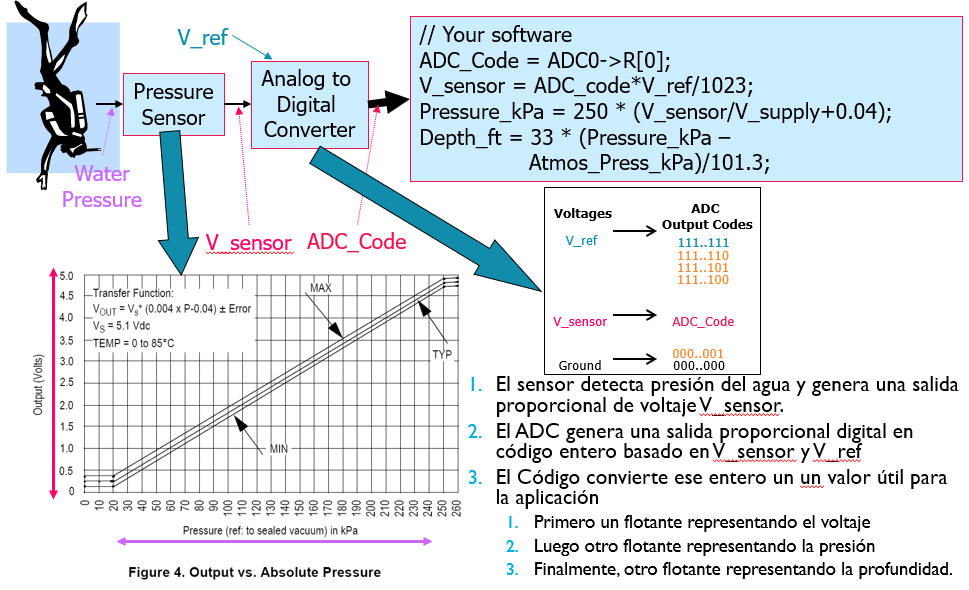
\includegraphics[scale=0.45]{fig_BigPicture}
	\end{figure}
\end{frame}
%%%%%%%%%%%%%%%%% FRAME %%%%%%%%%%%%%%%%%%%%%%%%%%
\begin{frame}
	\frametitle{Obteniendo de análogo a digital}
	\begin{columns}
		\column{0.7\linewidth}
		\begin{itemize}
			\setlength\itemsep{1.5cm}
			\item Un comparador nos dice si $V_{in}>V_{ref}$.
			\begin{itemize}
				\item Se compara un \textbf{voltaje análogo de entrada} con un \textbf{voltaje de referencia} para determinar cual es mas grande, retornando un bit 1. 
				\item Indicar si la profundidad es mayor a 100 m.
				\item Poner $V_{ref}$ al voltaje que marca dicha presión. 
			\end{itemize}
			\item Un convertidor de análogo a digital (ADC) nos dice que tan grande es $V_{in}$ en comparación de $V_{ref}$.
			\begin{itemize}
				\item Lee una señal análoga y produce el correspondiente numero bit binario a la salida. 
			\end{itemize}
		\end{itemize}
	
		\column{0.3\linewidth}
		\begin{figure}
			\centering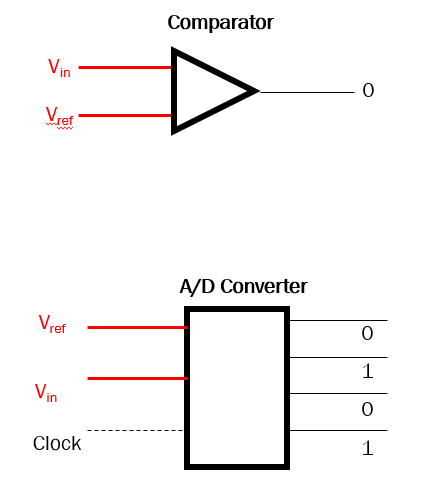
\includegraphics[scale=0.45]{fig_ComparatorADC}
		\end{figure}
	\end{columns}
\end{frame}
%%%%%%%%%%%%%%%%% FRAME %%%%%%%%%%%%%%%%%%%%%%%%%%
\begin{frame}
	\frametitle{Conversión de digital a análogo}
	\begin{columns}
		\column{0.7\linewidth}
		\begin{itemize}
			\setlength\itemsep{0.5cm}
			\item Se necesita generar un voltaje análogo o corriente como una señal de salida. 
			\begin{itemize}
				\item Ejemplo: señal de audio, señal de intensidad de brillo.
			\end{itemize}
			\item DAC: Generar un voltaje análogo como una fracción del voltaje de referencia.
			\item Ecuación de conversión entre digital a análogo. 
			\begin{itemize}
				\item $n$ código de entrada.
				\item $N$ número de bits de resolución.
				\item $V_{ref}$ voltaje de referencia.
				\item $V_{out}$ voltaje de salida. Esta dado por $V_{out}=V_{ref}*n/2^N$
 			\end{itemize}
		\end{itemize}
		
		\column{0.3\linewidth}
		{\vspace{2cm}}
		\begin{figure}
			\centering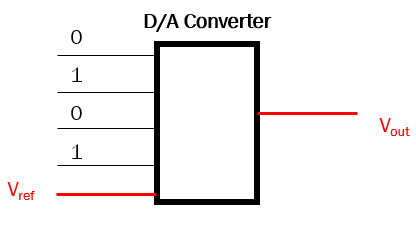
\includegraphics[scale=0.45]{fig_DACConverter}
		\end{figure}
	\end{columns}
\end{frame}
%%%%%%%%%%%%%%%%% FRAME %%%%%%%%%%%%%%%%%%%%%%%%%%
\begin{frame}
	\frametitle{Muestreo y cuantización de una señal}
	
	\begin{figure}
		\centering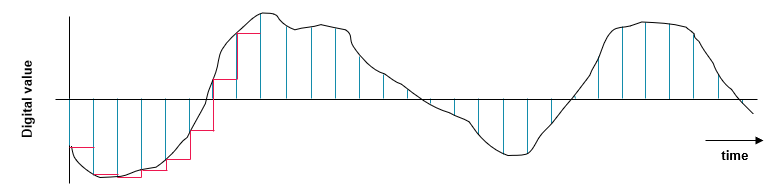
\includegraphics[scale=0.45]{fig_Sampling}
	\end{figure}
	
	\begin{itemize}
		\item Una señal es muestreada a un frecuencia constante cada $\delta t$.
		\begin{itemize}
			\item Cada muestra representa un valor instanteneo de amplitud en dicho instante.
			\item A los \SI{37}{\milli\second}, la entrada tiene el valor \SI{1.913419214124}{\volt}
			\item Muestrear convierte una señal en tiempo continuo a valores discretos. 
		\end{itemize}
		\item La muestra puede ahora ser cuantizada en un valor digital.
		\begin{itemize}
			\item La cuantización consiste en representar un valor continuo (análogo) con el valor más cercano discreto. 
			\item El valor de voltaje de entrada \SI{1.913419214124}{\volt} se puede representar con el código $0\times018$, ya que se encuentra entre el rango \SI{1.901}{\volt} a \SI{1.998}{\volt} el cual corresponde a dicho código. 
		\end{itemize}
	\end{itemize}
\end{frame}
%%%%%%%%%%%%%%%%% FRAME %%%%%%%%%%%%%%%%%%%%%%%%%%
\begin{frame}
	\frametitle{Como se obtiene el valor o código de $n$ para representar el voltaje de entrada en el ADC?}
	{\small
		
		La ecuación general está dada por
		%
		$$n = \floor*{\frac{(V_{in}-V_{-ref})2^N}{V_{+ref}-V_{-ref}}+1/2}$$
		%
		donde $n$ es el código, $V_{in}$ el voltaje de entrada, $V_{+ref}$ voltaje de referencia superior, $V_{-ref}$ voltaje de referencia inferior, y $N$ el número de bits. Por lo general el voltaje de referencia inferior es \SI{0}{\volt}, entonces
		%
		$$n = \floor*{\frac{V_{in}2^N}{V_{+ref}}+1/2}$$
		
		\textbf{Ejemplo}: suponga que se tiene un convertidor ADC de 10 bits, el voltaje de referencia es de \SI{5}{\volt}, y el de entrada es de \SI{3.3}{\volt}, obtenga el código de salida. Aplicando la formula se tiene que
		%
		$$n = \floor*{\frac{\SI{3.3}{\volt} \ 2^{10}}{\SI{5}{\volt}}+1/2} = 676$$
}	
\end{frame}
%%%%%%%%%%%%%%%%% FRAME %%%%%%%%%%%%%%%%%%%%%%%%%%
\begin{frame}
	\frametitle{Conceptos del ADC - Convertidor Flash }
	{\small
		\begin{columns}
			\column{0.5\linewidth}
			\begin{itemize}
				\setlength\itemsep{0cm}
				\item Un divisor multinivel de voltaje es usado para poner la salida sobre todo el rango de conversión.
				\item Un comparador es usado en cada nivel para determinar si el voltaje es inferior o superior en dicho nivel.
				\item La salida de los comparadores son codificadas en número binarios con prioridad. 
				\item Componentes usados: $2^N$ resistencia, y $2^N-1$ comparadores.
				\item Nota:
				\begin{itemize}
					\item El divisor de resistencias genera un voltaje el cual no satisface $1/2$ bit, lo que ocasiona un error de un bit.
					\item Se puede cambiar el offset con los valores de las resistencias. 
				\end{itemize}
			\end{itemize}
			
			\column{0.5\linewidth}
			\begin{figure}
				\centering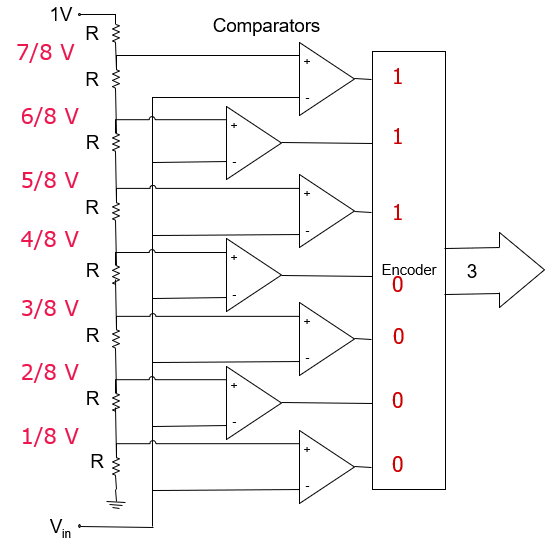
\includegraphics[scale=0.45]{fig_FlashComparator}
			\end{figure}
		
		\end{columns}
	}	
\end{frame}
%%%%%%%%%%%%%%%%% FRAME %%%%%%%%%%%%%%%%%%%%%%%%%%
\begin{frame}
	\frametitle{Conceptos del ADC - Convertidor de aproximaciones sucesivas (SAR)}
	{\small
		\begin{columns}
			\column{0.5\linewidth}
			\begin{itemize}
				\setlength\itemsep{0cm}
				\item Se aproxima sucesivamente el voltaje de entrada realizando una búsqueda binaria y un DAC. 
				\item El registro SA almacena el valor actual de la aproximación.
				\item Se pone todas las entradas del DAC en cero.
				\item Pone un uno en el bit más significativo del DAC.
				\item Se repite
				\begin{itemize}
					\item Poner el siguiente bit del DAC en 1.
					\item Esperar a que se estabilice y comparar el DAC con la salida.
					\item Si la salida del DAC es menor que la entrada entonces se pone el siguiente bit en 1, sino se el bit actual en cero. 
				\end{itemize}
			\end{itemize}
			
			\column{0.5\linewidth}
			\begin{figure}
				\centering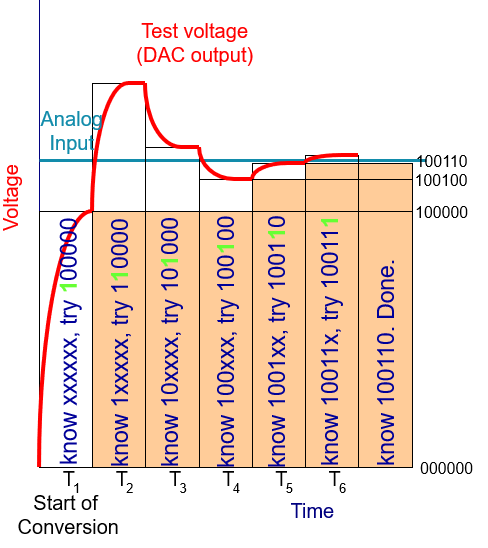
\includegraphics[scale=0.45]{fig_SARConversion}
			\end{figure}
			
		\end{columns}
	}	
\end{frame}
%%%%%%%%%%%%%%%%% FRAME %%%%%%%%%%%%%%%%%%%%%%%%%%
\begin{frame}
	\frametitle{Esquemático del SAR}
	\begin{figure}
		\centering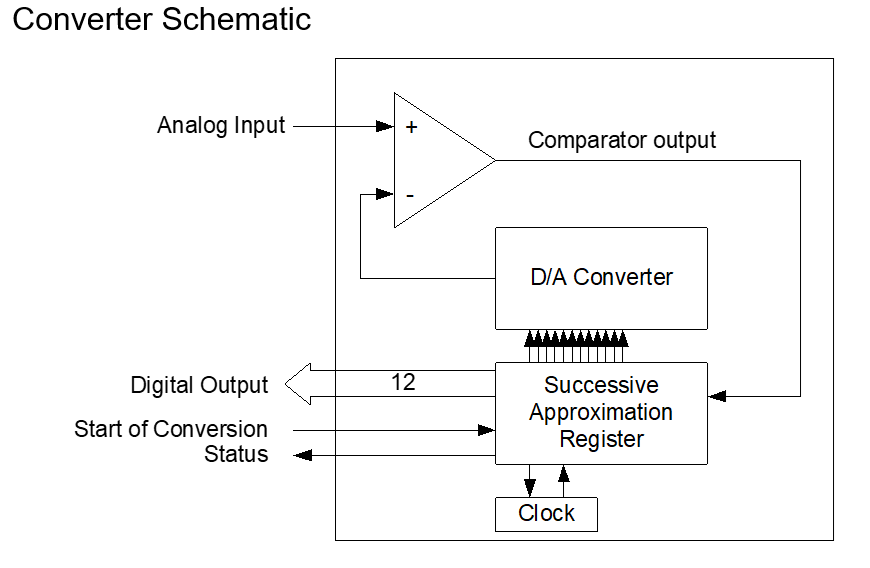
\includegraphics[scale=0.45]{fig_SARSchematic}
	\end{figure}
\end{frame}
%%%%%%%%%%%%%%%%% FRAME %%%%%%%%%%%%%%%%%%%%%%%%%%
\begin{frame}
	\frametitle{Conceptos del ADC - Métrica y problemas}
	{\small
		\begin{itemize}
			\item La \textbf{linealidad} mide que tanto la conversión se mantiene en una linea recta.
			\item \textbf{Linealidad diferencial} mide la igualdad entre pasos.
			\item \textbf{Tiempo de conversión}: desde que se comienza la conversión hasta que está listo el resultado.
			\item \textbf{Tasa de conversión}: inverso del tiempo. 
		\end{itemize}
	
		Cuando se muestrea una señal analógica se debe tener en cuenta los siguiente problemas.
		%
		\begin{itemize}
			\item \textbf{Criterio de Nyquist}: muestrear al menos 2 veces más rápido que la señal para poder reconstruirla. 
			\item Este criterio asume que se tienen filtro perfecto.
			\item Se debe elegir una frecuencia de muestreo mayor para atenuar efectos de aliasing. 
		\end{itemize}
	}	
\end{frame}
%%%%%%%%%%%%%%%%% FRAME %%%%%%%%%%%%%%%%%%%%%%%%%%
\begin{frame}
	\frametitle{Dispositivos de muestreo y retención}
	{\small
		\begin{figure}
			\centering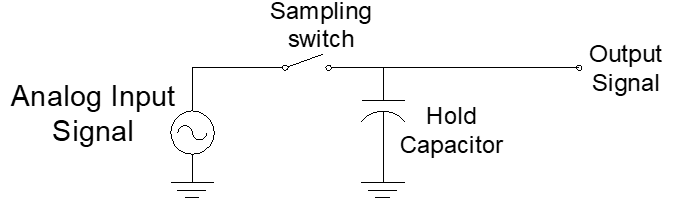
\includegraphics[scale=0.5]{fig_SampleHold}
		\end{figure}
		
		\begin{itemize}
			\item Algunos convertidores ADC requieren que la entrada se mantenga constante durante la conversión (ej: SAR).
			\item En otros casos, la captura del pico o el muestreo a un punto específico requiere de un circuito adicional.
			\item Muchos de los ADC contienen dicho circuito. 
		\end{itemize}
	}	
\end{frame}
%%%%%%%%%%%%%%%%% FRAME %%%%%%%%%%%%%%%%%%%%%%%%%%
\begin{frame}
	\frametitle{Pines del K64}
	{\small
		\begin{columns}
			\column{0.5\linewidth}
			\begin{itemize}
				\item 100 LQFP
				\item 2 ADC de 16-bit ADC con hasta 14 canales. 
				\item 2 comparadores.
				\item 1 DAC de 12-bits
			\end{itemize}
			
			\column{0.5\linewidth}
			\begin{figure}
				\centering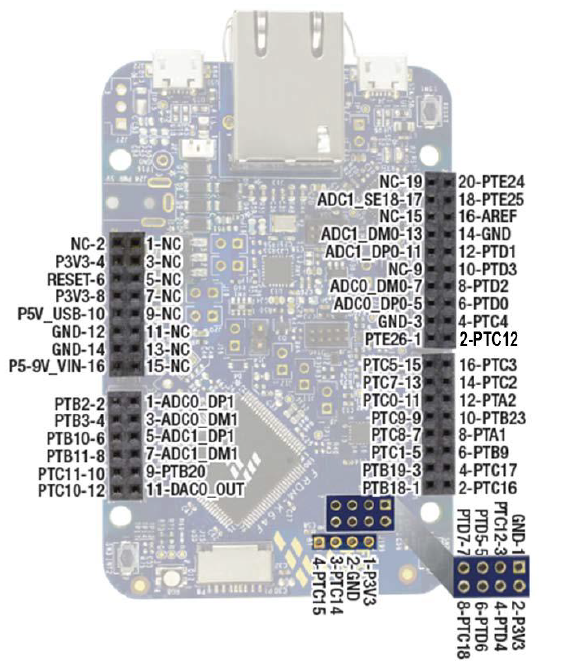
\includegraphics[scale=0.4]{fig_FRDMPinout}
			\end{figure}
			
		\end{columns}
	}	
\end{frame}
%%%%%%%%%%%%%%%%% FRAME %%%%%%%%%%%%%%%%%%%%%%%%%%
\begin{frame}
	\frametitle{Usar el pin como entrada o salida análoga}
	{\small
		\begin{columns}
			\column{0.5\linewidth}
			\begin{itemize}
				\item Recuerde configurar con el registro PCR, tanto dirección como MUX.
				\item Dato: la salida hay diferentes formas para acceder, y la entrada existe el registro. 
			\end{itemize}
			
			\column{0.5\linewidth}
			\begin{figure}
				\centering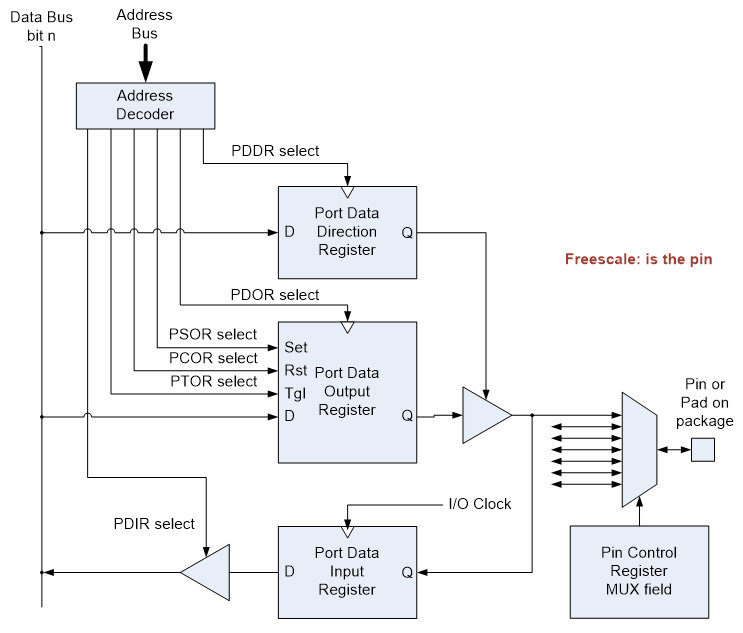
\includegraphics[scale=0.35]{fig_PCR}
			\end{figure}
			
		\end{columns}
	}	
\end{frame}
%%%%%%%%%%%%%%%%% FRAME %%%%%%%%%%%%%%%%%%%%%%%%%%
\begin{frame}
	\frametitle{Registro de control de pin PCRn}
	\begin{figure}
		\centering
		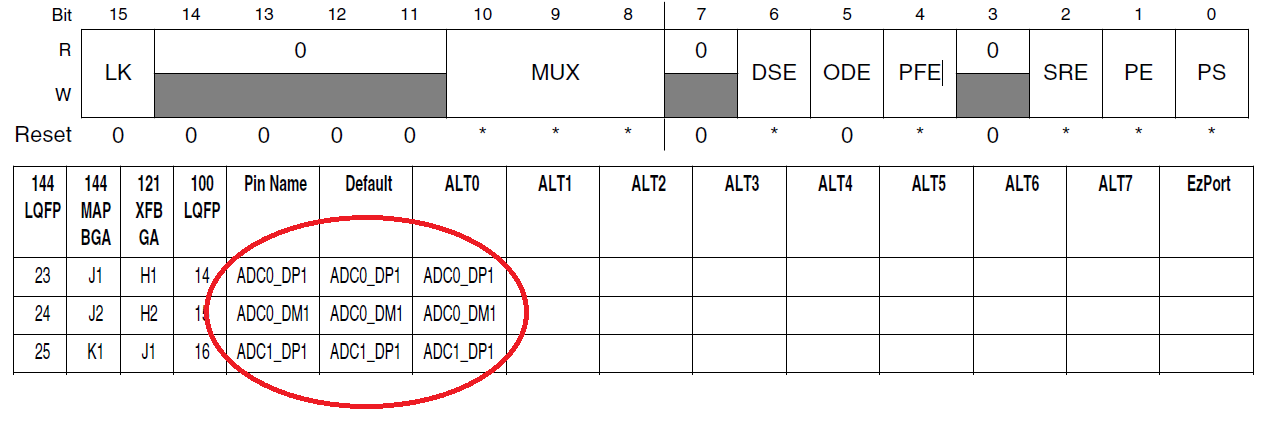
\includegraphics[scale=0.4]{fig_PCR2}
	\end{figure}
	\begin{columns}
		\column{0.5\linewidth}
		El campo del MUX define las conexiones internas de la señal.
		\column{0.5\linewidth}
		\begin{scriptsize}
			\begin{tabular}{ cc } 
				\hline
				\textbf{MUX (bit 10-8)} & \textbf{Configuración}  \\ 
				\hline
				000 & Pin deshabilitado  \\ 
				001 & ALT 1 - GPIO \\ 
				010 & ALT 2 \\ 
				011 & ALT 3 \\ 
				100 & ALT 4 \\ 
				101 & ALT 5 \\ 
				110 & ALT 6 \\ 
				111 & ALT 7 \\ 
				\hline
			\end{tabular}
		\end{scriptsize}
	\end{columns}
\end{frame}
%%%%%%%%%%%%%%%%% FRAME %%%%%%%%%%%%%%%%%%%%%%%%%%
\begin{frame}
	\frametitle{Conversor digital a análogo (DAC)}
	\begin{figure}
		\centering
		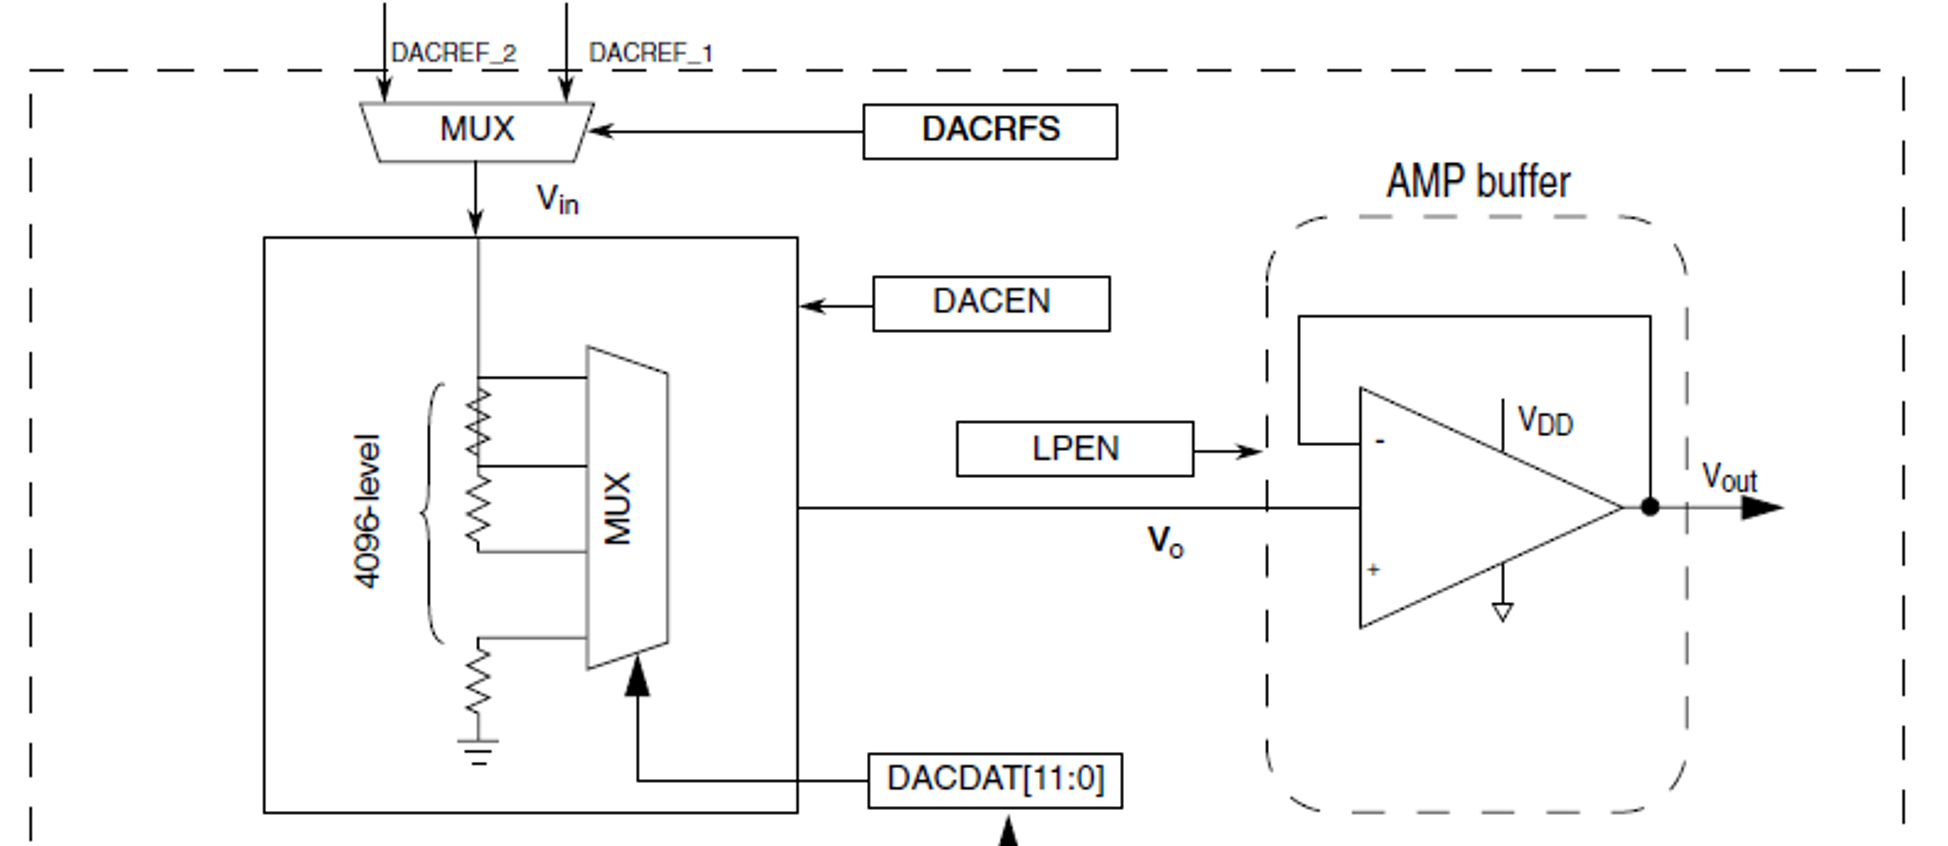
\includegraphics[scale=0.25]{fig_DACSchematic}
	\end{figure}
	\begin{itemize}
		\item Cargar en el registro DACDAT con un dato de 12-bit.
		\item El MUX selecciona un nodo de la red de resistencia para crear la salida dada por $V_o = (N+1)V_{in}/2^{12}$.
		\item $V_o$ es acoplado a la salida por el amplificador operacional. 
	\end{itemize}
\end{frame}
%%%%%%%%%%%%%%%%% FRAME %%%%%%%%%%%%%%%%%%%%%%%%%%
\begin{frame}
	\frametitle{Modos de operación del DAC}
	 \begin{itemize}
	 	\item Normal
	 	\begin{itemize}
	 		\item DAT0 es convertido a salida de voltaje inmediatamente.
	 	\end{itemize}
	 	\item Buffered
	 	\begin{itemize}
	 		\item Los datos a la salida son almacenados en un buffer de 16 bits.
	 		\item El siguiente dato es enviado al DAC cuando ocurre un evento por disparo. 
	 		\begin{itemize}
	 			\item Evento por software - escribir al campo DACSWTRG en el DACx\_C0
	 			\item Evento por hardware - del timer. 
	 		\end{itemize}
 		\item Modo normal - buffer circular
 		\item Modo de escaneo una única vez
 		\item Bandera de estatus en DACx\_SR
	 	\end{itemize}
	 \end{itemize}
\end{frame}
%%%%%%%%%%%%%%%%% FRAME %%%%%%%%%%%%%%%%%%%%%%%%%%
\begin{frame}
	\frametitle{Registro de control 0 para el DAC (DACx\_C0)}
	{\small
	\begin{figure}
		\centering
		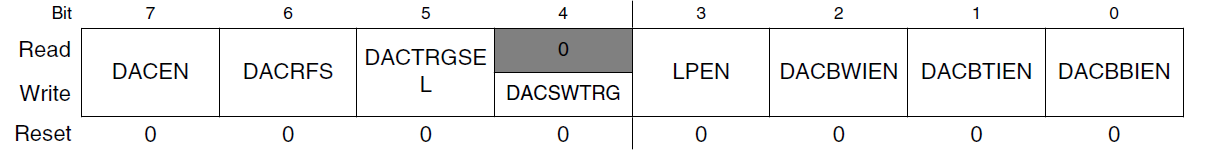
\includegraphics[scale=0.5]{fig_DACxC0}
	\end{figure}
	\begin{columns}
		\column{0.7\linewidth}
		\begin{itemize}
			\setlength\itemsep{0em}
			\item DACEN - habilita el DAC cuando es un 1.
			\item DACRFS - seleccionar la referencia de voltaje para el DAC.
			\begin{itemize}
				\item 0: DACREF\_1 conectado a VREFH
				\item 1: DACREF\_2 conectado al VDDA
			\end{itemize}
			\item LPEN - modo de bajo consumo.
			\begin{itemize}
				\item 0: modo de alta velocidad. Rápido (\SI{15}{\micro\second} tiempo de asentamiento), pero usa mayor potencia. 
				\item 1: modo bajo consumo. Lento (\SI{100}{\micro\second}) pero menos potencia. 
			\end{itemize}
			\item Registros adicional para el control en modo buffered. 
		\end{itemize}
		
		\column{0.3\linewidth}
		\begin{figure}
			\centering
			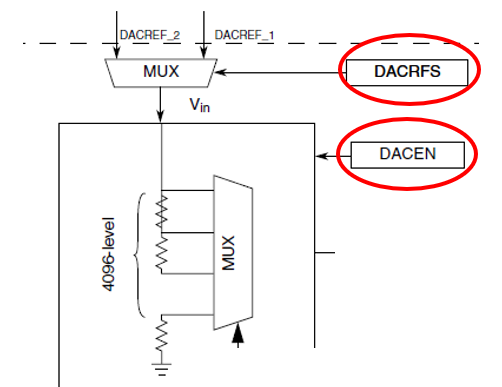
\includegraphics[scale=0.5]{fig_DACxC0Schematic}
		\end{figure}
	\end{columns}
	}
\end{frame}
%%%%%%%%%%%%%%%%% FRAME %%%%%%%%%%%%%%%%%%%%%%%%%%
\begin{frame}
	\frametitle{Registro de control 1 para el DAC (DACx\_C1)}
	{\small
		\begin{figure}
			\centering
			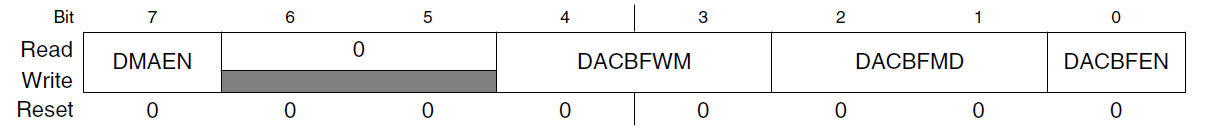
\includegraphics[scale=0.7]{fig_DACxC1}
		\end{figure}
		\begin{itemize}
			\item DACBFEN:
			\begin{itemize}
				\item 0: Deshabilita el modo buffer.
				\item 1: Habilita el modo buffer.
			\end{itemize}
			\item DACBFMD - selecciona el modo buffer.
			\begin{itemize}
				\item 0: Modo normal
				\item 1: Modo de un solo escaneo. 
			\end{itemize}
		\end{itemize}	
	}
\end{frame}
%%%%%%%%%%%%%%%%% FRAME %%%%%%%%%%%%%%%%%%%%%%%%%%
\begin{frame}
	\frametitle{Registro de datos para el DAC}
	{\small
		\begin{itemize}
			\item Estos registros son solo de 8 bits.
			\item DATA[11:0] se almacena en dos registros.
			\begin{itemize}
				\item DATA0: byte bajo en DACx\_DATnL
				\item DATA1: nibble alto en DACx\_DATnH
			\end{itemize}
		\end{itemize}
	
	\textbf{Pasos para trabajar con el DAC}
	
	 \begin{itemize}
	 	\setlength\itemsep{0em}
	 	\item Habilite el clock del DAC
	 	\item Ponga el MUX del PCR para trabajar análogo.
	 	\item Habilite el DAC
	 	\item Configure el DAC: voltaje de referencia, bajo consumo, modo normal.
	 	\item Escriba el registro del DAC
	 \end{itemize}
	}
\end{frame}
%%%%%%%%%%%%%%%%% FRAME %%%%%%%%%%%%%%%%%%%%%%%%%%
\begin{frame}[fragile]
	\frametitle{Ejemplo - DAC}
	{\small
		Genere una señal de salida triangular utilizando el DAC.
		\begin{lstlisting}[style=CStyle]
void Init_DAC(void) {
	// Enable clock to DAC
	//SIM->SCGC6 |= SIM_SCGC6_DAC0_MASK;
	SIM->SCGC2 |= SIM_SCGC2_DAC0_MASK;
	
	// Disable buffer mode
	DAC0->C1 = (uint8_t)0;
	
	// Enable DAC, select VDDA as reference voltage
	DAC0->C0 = (uint8_t)(DAC_C0_DACEN_MASK | DAC_C0_DACRFS_MASK);
}
		\end{lstlisting}
	}
\end{frame}
%%%%%%%%%%%%%%%%% FRAME %%%%%%%%%%%%%%%%%%%%%%%%%%
\begin{frame}[fragile]
	\frametitle{Ejemplo - DAC}
	{\small
		Genere una señal de salida triangular utilizando el DAC.
		\begin{lstlisting}[style=CStyle]
void Triangle_Output(void) {
	int i=0, change=1;
	
	while (1) {
		DAC0->DAT[0].DATL = DAC_DATL_DATA0(i);
		DAC0->DAT[0].DATH = DAC_DATH_DATA1(i >> 8);
		
		i += change;
		if (i == 0) {
			change = 1;
		} else if (i == DAC_RESOLUTION-1) {
			change = -1;
		}
	}
}
		\end{lstlisting}
	}
\end{frame}
%%%%%%%%%%%%%%%%% FRAME %%%%%%%%%%%%%%%%%%%%%%%%%%
\begin{frame}[fragile]
	\frametitle{Panorama general del ADC}
	{\small
		\begin{itemize}
			\item Usa aproximaciones sucesivas para la conversión.
			\item Soporta múltiples resoluciones: 16, 12, 8 bit. 
			\item Soporta conversiones diferenciales o de un solo canal.
			\item Comparación automática e interrupción por nivel.
			\item Promedio de datos por hardware.
			\item Sensor de temperatura.
		\end{itemize}
	}
\end{frame}
%%%%%%%%%%%%%%%%% FRAME %%%%%%%%%%%%%%%%%%%%%%%%%%
\begin{frame}[fragile]
	\frametitle{Sistema general del ADC}
	{\small
		\begin{columns}
			\column{0.5\linewidth}
			\begin{itemize}
				\item Inicialización del ADC
				\begin{itemize}
					\item Configurar el clock
					\item Seleccionar el voltaje de referencia a trabajar.
					\item Seleccionar la fuente de trigger.
					\item Seleccionar el canal.
					\item Seleccionar otros parámetros.
				\end{itemize}
				\item Disparar la conversión.
				\item Leer resultados. 
			\end{itemize}
			
			\column{0.5\linewidth}
			\begin{figure}
				\centering
				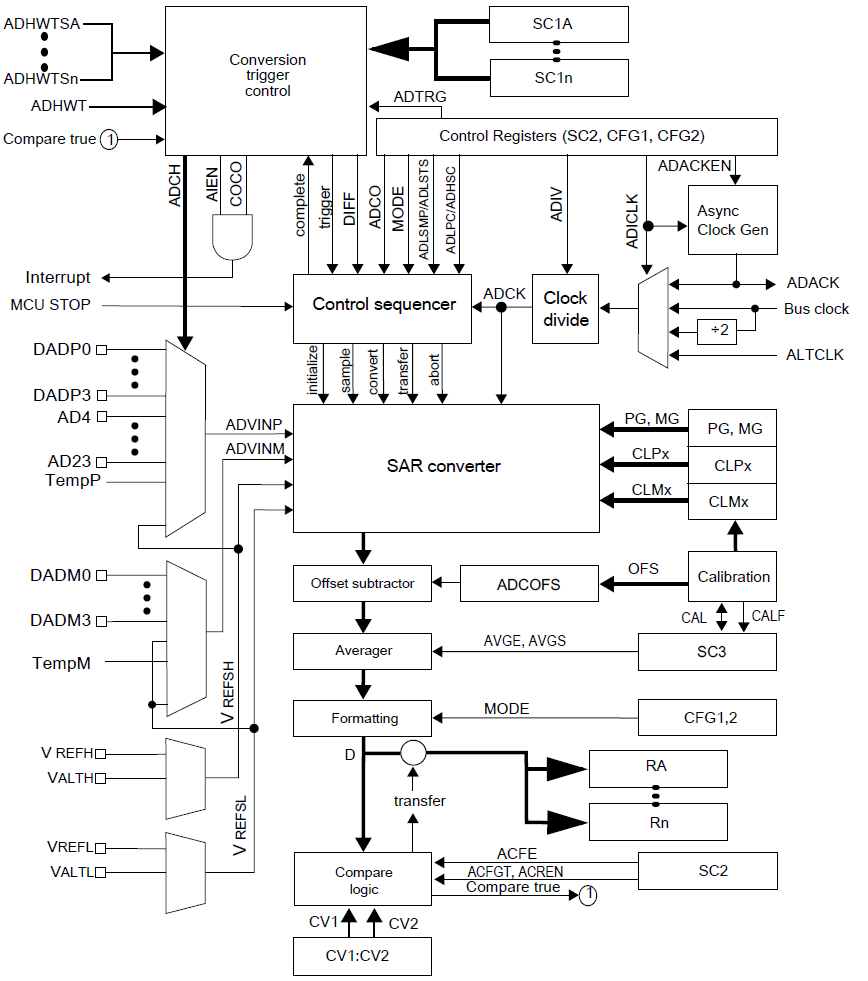
\includegraphics[scale=0.4]{fig_SAR}
			\end{figure}
		\end{columns}
	}
\end{frame}
%%%%%%%%%%%%%%%%% FRAME %%%%%%%%%%%%%%%%%%%%%%%%%%
\begin{frame}[fragile]
	\frametitle{Configuración del clock}
	{\small
		\begin{columns}
			\column{0.5\linewidth}
			\begin{itemize}
				\item Seleccione la fuente del clock ADICLK
				\begin{itemize}
					\item Bus clock.
					\item ADACK: clock local, permite operaciones del ADC mientras la CPU está parada.
					\item ALTCLK: clock alternativo
				\end{itemize}
				\item Divide el clock seleccionado por un factor de ADIV, creando asi ADCK.
				\item El ADCK resultante debe estar en un rango valido, que depende de las resolución. 
			\end{itemize}
			
			\column{0.5\linewidth}
			\begin{figure}
				\centering
				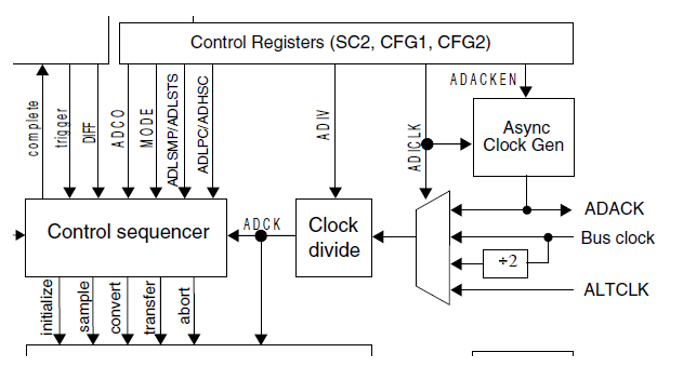
\includegraphics[scale=0.5]{fig_ClockADC}
			\end{figure}
		\end{columns}
	}
\end{frame}
%%%%%%%%%%%%%%%%% FRAME %%%%%%%%%%%%%%%%%%%%%%%%%%
\begin{frame}
	\frametitle{Registros para configuración del clock}
	{\small
		\begin{columns}
			\column{0.5\linewidth}
			\begin{itemize}
				\item ADCx\_CGF1
				\begin{itemize}
					\item ADIV: divide el clock por $2^{ADIV}$
					\item ADICLK: selección del bus de entrada.
					\begin{itemize}
						\item 00: bus clock
						\item 01: bus clock/2
						\item 10: ALTCLK
						\item 11: ADACK
					\end{itemize}
				\end{itemize}
				\item ADCx\_CGF2 
				\begin{itemize}
					\item ADACKEN: habilita clock asíncrono. 
				\end{itemize}
			\end{itemize}
			
			\column{0.5\linewidth}
			\begin{figure}
				\centering
				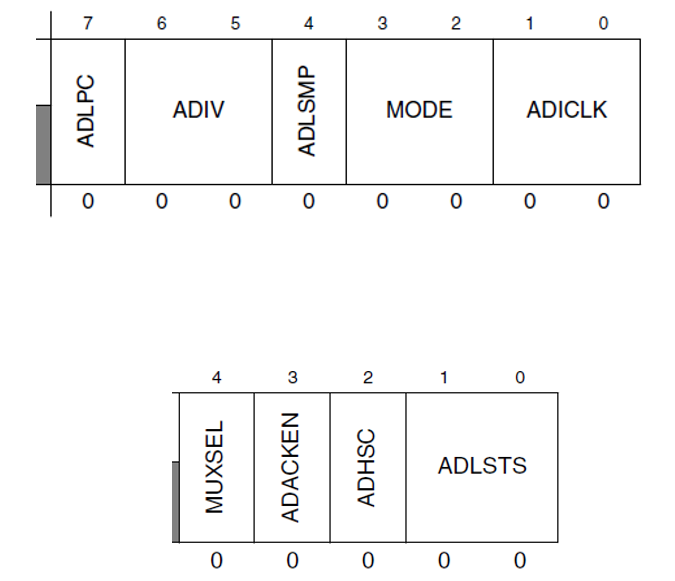
\includegraphics[scale=0.4]{fig_ADCRegister}
			\end{figure}
		\end{columns}
	}
\end{frame}
%%%%%%%%%%%%%%%%% FRAME %%%%%%%%%%%%%%%%%%%%%%%%%%
\begin{frame}
	\frametitle{Selección del voltaje de referencia}
	{\small
		\begin{columns}
			\column{0.5\linewidth}
			\begin{itemize}
				\item Dos pares de voltaje de referencia estan disponibles
				\begin{itemize}
					\item $V_{REFH}, V_{REFL}$
					\item $V_{ALTH}, V_{ALTL}$
				\end{itemize}
				\item Dentro del registro SC2 el campo de bits REFSEL
				\begin{itemize}
					\item 00: $V_{REFH}, V_{REFL}$
					\item 01: $V_{ALTH}, V_{ALTL}$
					\item 10, 11: reservado
				\end{itemize}
				\item K64
				\begin{itemize}
					\item $V_{ALTH}$ conectado a $V_{DDA}$
				\end{itemize}
			\end{itemize}
			
			\column{0.5\linewidth}
			\begin{figure}
				\centering
				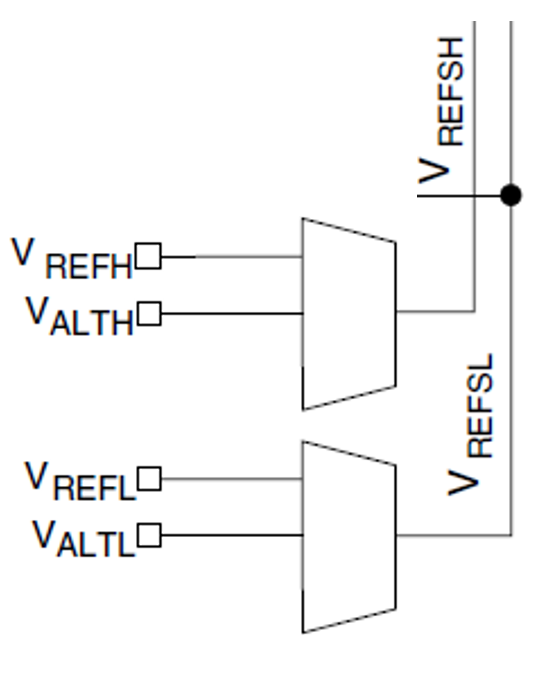
\includegraphics[scale=0.4]{fig_VoltageReference}
			\end{figure}
		\end{columns}
	}
\end{frame}
%%%%%%%%%%%%%%%%% FRAME %%%%%%%%%%%%%%%%%%%%%%%%%%
\begin{frame}
	\frametitle{Selección del trigger para la conversión}
	{\small
		\begin{columns}
			\column{0.5\linewidth}
			\begin{itemize}
				\item ADTRG en SC2
				\begin{itemize}
					\item 0: trigger por software
					\item 1: trigger por hardware
				\end{itemize}
				\item Trigger por software
				\begin{itemize}
					\item Escribir al SCIA
				\end{itemize}
				\item Buffering ping-pong
				\begin{itemize}
					\item SCIA vs SCIn
				\end{itemize}
				\item Trigger por hardware
				\begin{itemize}
					\item Flanco de subida para la señal ADHWT
					\item Fuente para el ADHWT: TPM, LPTMR, PIT, RTC, EXTRG\_IN
				\end{itemize}
			\end{itemize}
			
			\column{0.5\linewidth}
			\begin{figure}
				\centering
				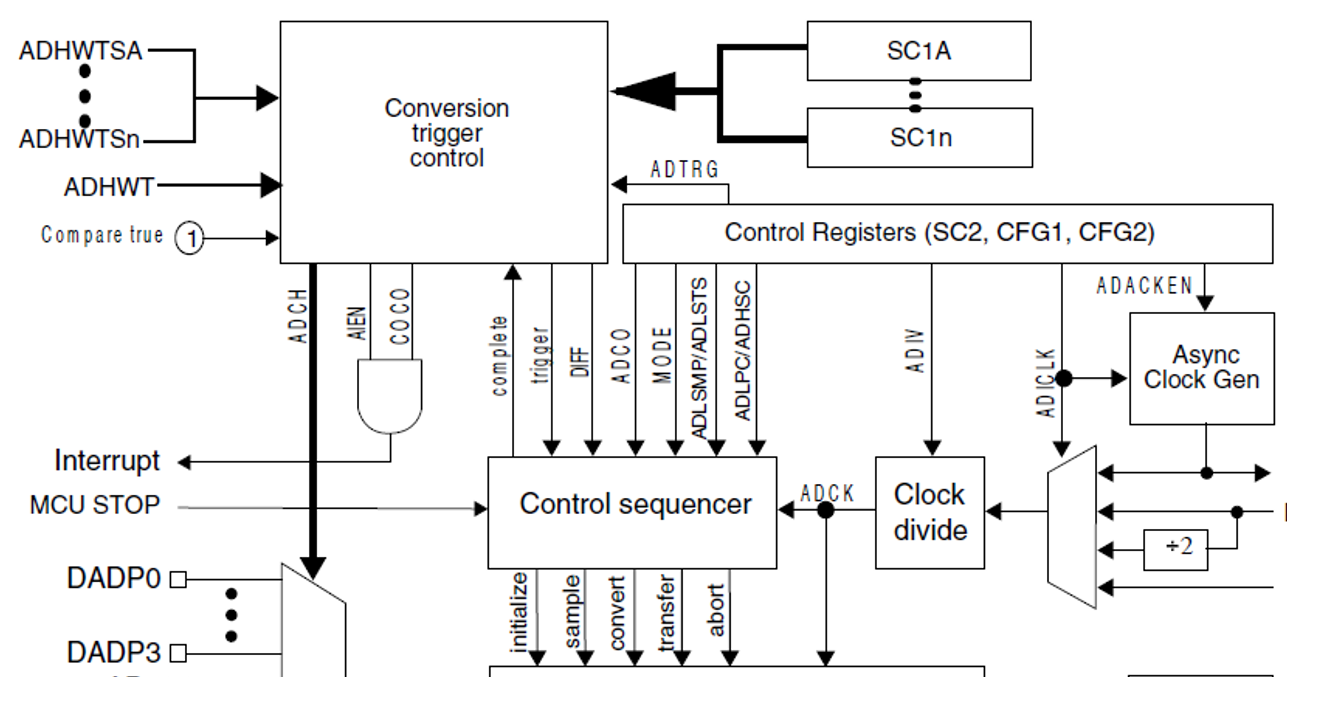
\includegraphics[scale=0.4]{fig_Trigger}
			\end{figure}
		\end{columns}
	}
\end{frame}
%%%%%%%%%%%%%%%%% FRAME %%%%%%%%%%%%%%%%%%%%%%%%%%
\begin{frame}
	\frametitle{Selección del modo de conversión}
	{\small
		\begin{columns}
			\column{0.6\linewidth}
			\begin{itemize}
				\setlength\itemsep{0em}
				\item Bajo consumo
				\begin{itemize}
					\item Poner ADLPC a 1 (en el ADCx\_CFG1)
					\item Velocidad máxima del reloj mas lenta.
				\end{itemize}
				\item Largo tiempo de muestreo
				\begin{itemize}
					\item Poner ADLSMP en 1 (en el ADCx\_CFG1)
					\item Se puede seleccionar tiempo de muestreo mas largos con ADLSTS
				\end{itemize}
				\item Modo de conversión
				\begin{itemize}
					\item Modo (en ADCx\_CFG1)
					\item Configurar la precisión del resultado (8 a 16 bits)
				\end{itemize}
				\item Conversión sencilla vs continua
				\begin{itemize}
					\item Poner en 1 el ADCO para conversión continua. 
				\end{itemize}
			\end{itemize}
			
			\column{0.4\linewidth}
			\begin{figure}
				\centering
				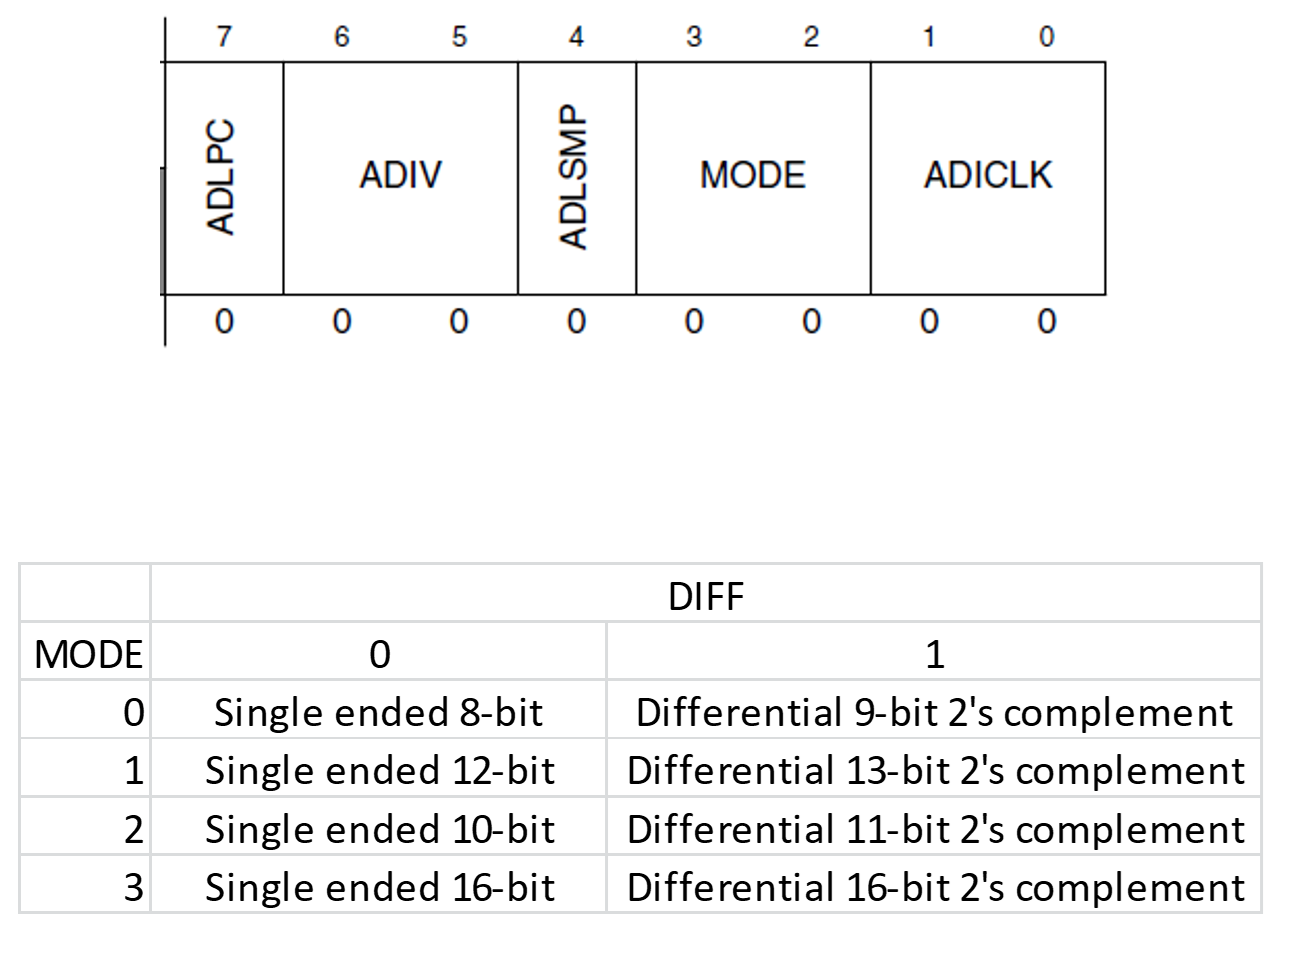
\includegraphics[scale=0.25]{fig_ADLS}
			\end{figure}
		\end{columns}
	}
\end{frame}
%%%%%%%%%%%%%%%%% FRAME %%%%%%%%%%%%%%%%%%%%%%%%%%
\begin{frame}
	\frametitle{Conversión completa}
	{\small
		\begin{figure}
			\centering
			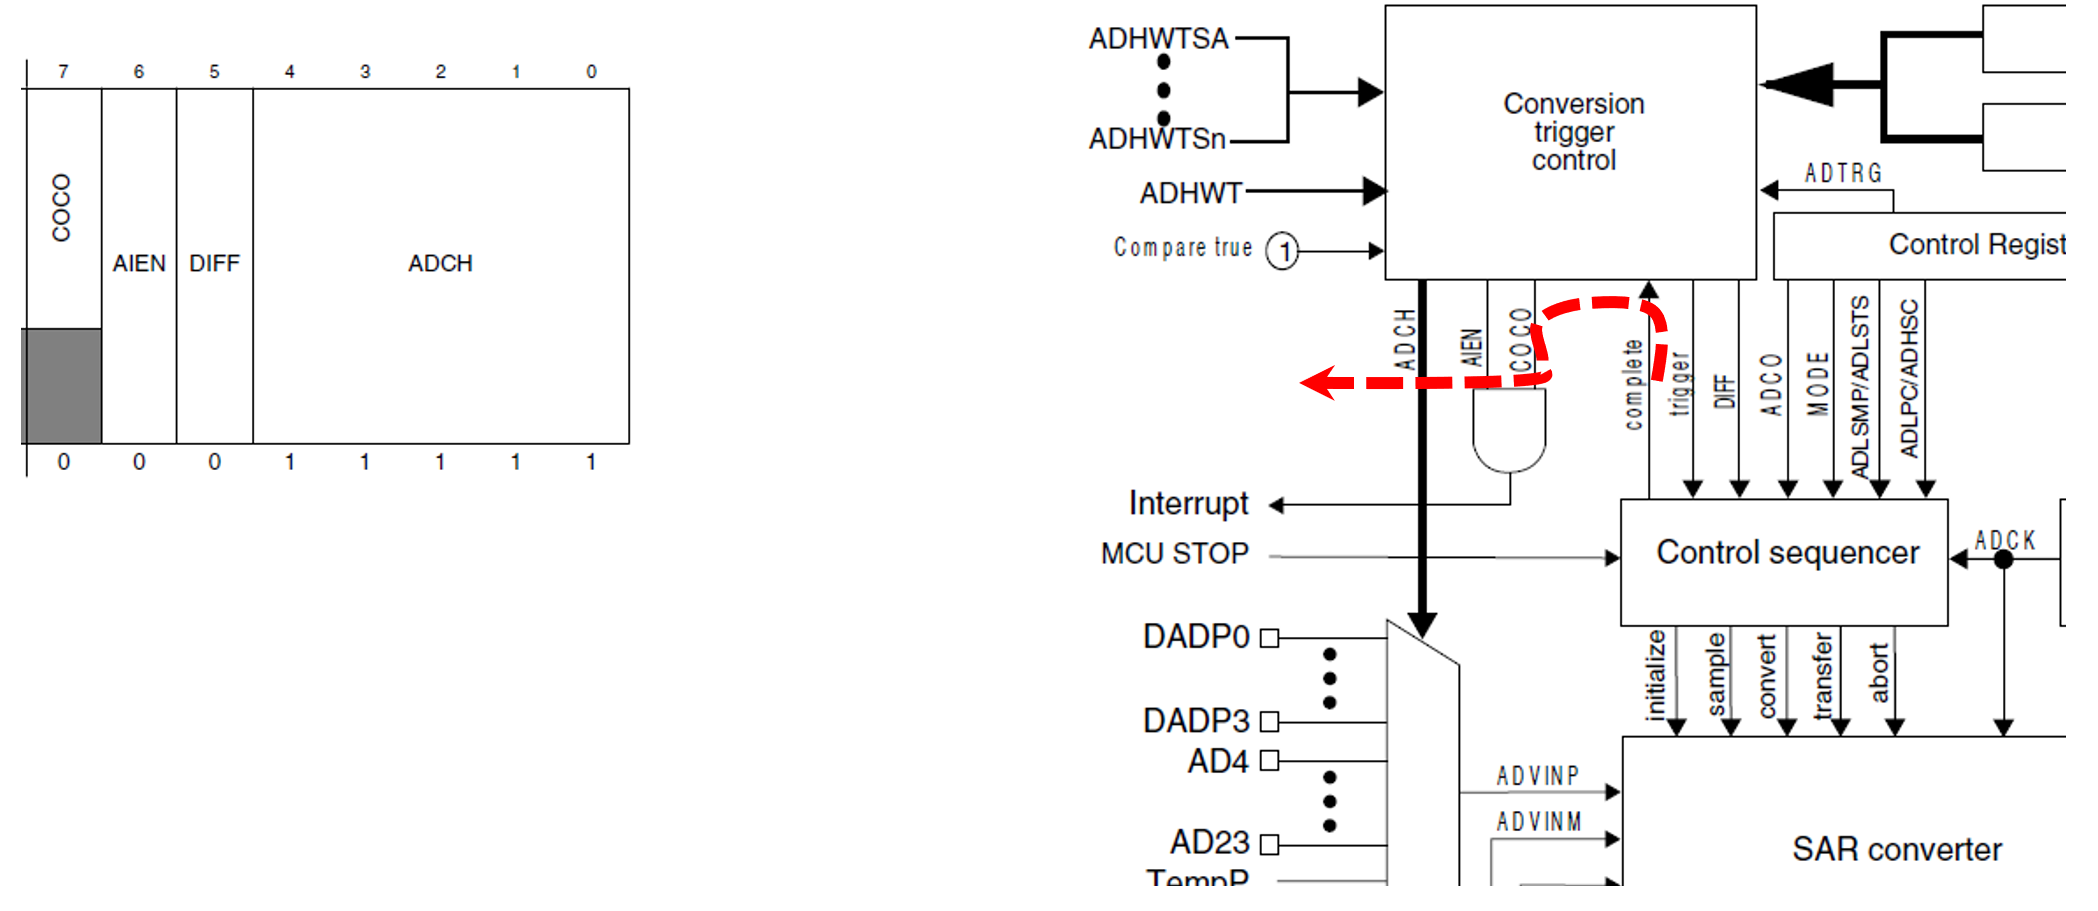
\includegraphics[scale=0.25]{fig_CompleteConversion}
		\end{figure}
		\begin{itemize}
			\item Señalada en el bit COCO del SCIn
			\item Puede generar una interrupción por conversión completa si AIEN en el SCI esta configurado.
			\begin{itemize}
				\item El handle del CMSIS para la interrupción se llama ADC0\_IRQHandler
			\end{itemize}  
		\end{itemize}	
	}
\end{frame}
%%%%%%%%%%%%%%%%% FRAME %%%%%%%%%%%%%%%%%%%%%%%%%%
\begin{frame}
	\frametitle{Registros del resultado}
	{\small
		\begin{columns}
			\column{0.6\linewidth}
			\begin{itemize}
				\setlength\itemsep{0em}
				\item Procesamiento adicional antes de ser almacenados en el registro de resultados
				\begin{itemize}
					\item Resta de offset de la calibración.
					\item Promediado: 1, 4, 8, 16 y 32 muestras.
					\item Formateo: justificación a la derecha, extensión de signo de 16 bits
					\item Comparación de salida
				\end{itemize}
				\item Dos registros de resultados RA y Rn 
				\begin{itemize}
					\item Resultado de la conversión para al registro correspondiente del SCI usado para iniciar la conversión
				\end{itemize}
			\end{itemize}
			
			\column{0.4\linewidth}
			\begin{figure}
				\centering
				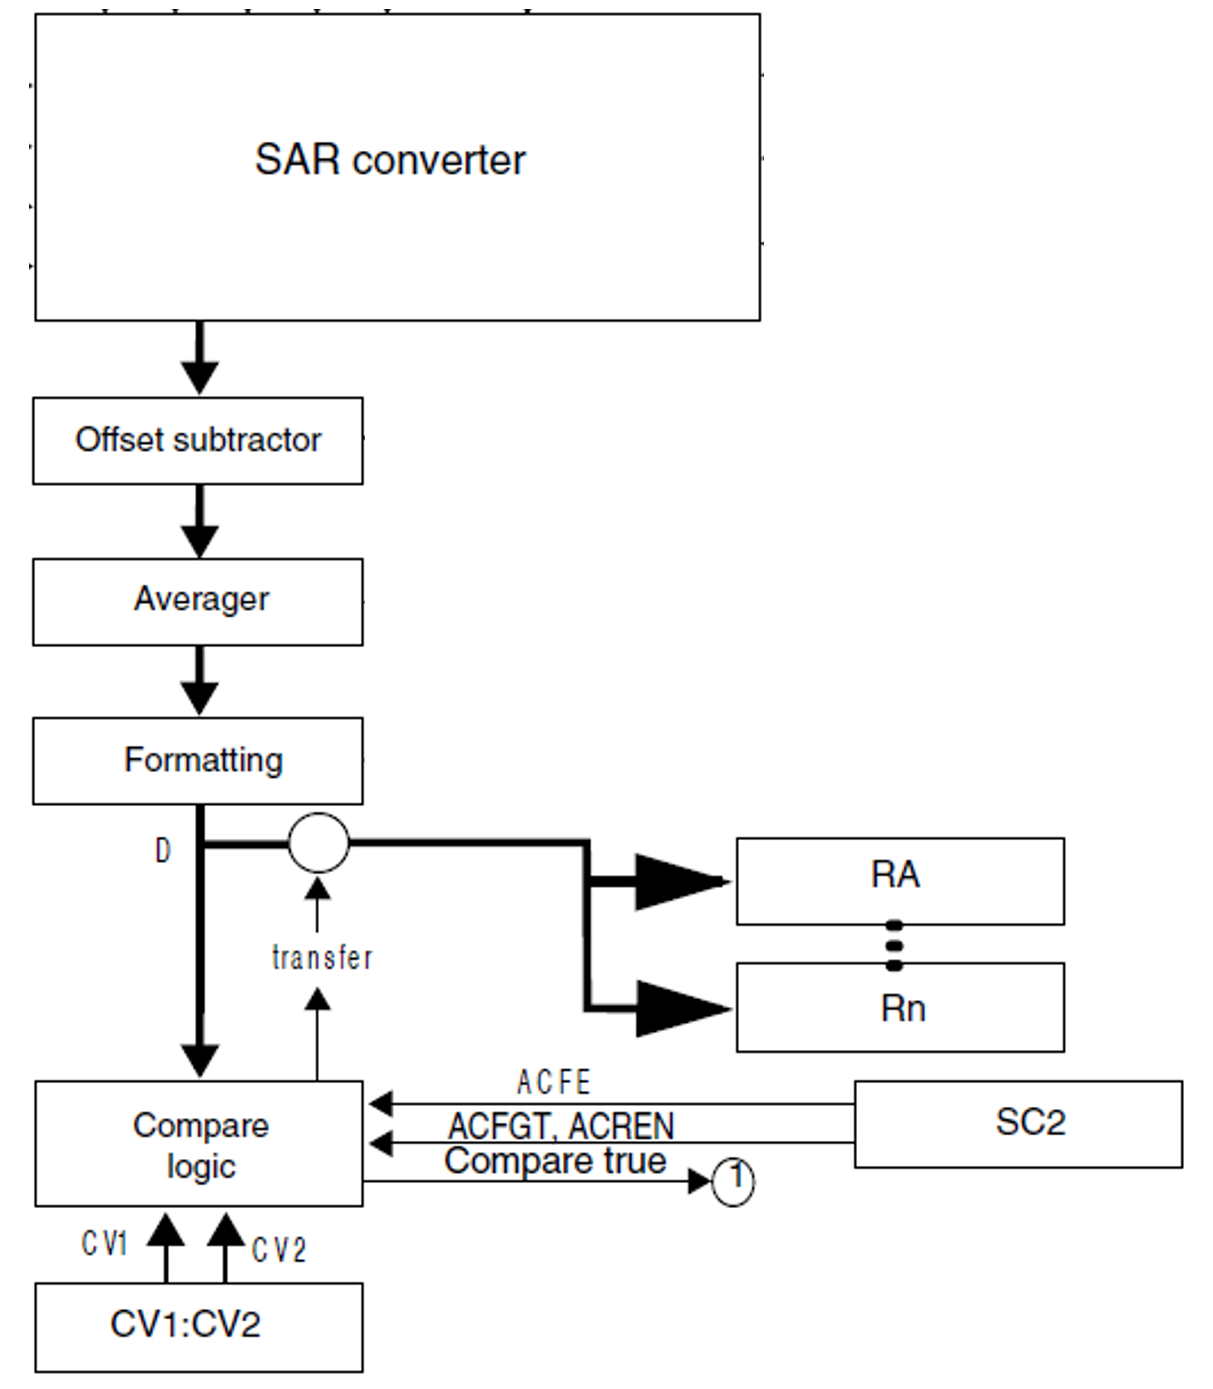
\includegraphics[scale=0.25]{fig_RegisterRA}
			\end{figure}
		\end{columns}
	}
\end{frame}
%%%%%%%%%%%%%%%%% FRAME %%%%%%%%%%%%%%%%%%%%%%%%%%
\begin{frame}[fragile]
	\frametitle{Ejemplo - Lectura de un potenciometro}
	{\small
		EL objetivo es utilizar un pin conversor de análogo a digital para hacer lectura del valor de voltaje de un potenciómetro. 
		
		\textbf{Solución}: primero se inicializa el ADC
\begin{lstlisting}[style=CStyle]
	#define ADC_CHANNEL (1)
	
	void Init_ADC(void) {
		
		SIM->SCGC6 |= SIM_SCGC6_ADC0_MASK;
		
		// Low power configuration, long sample time, 16 bit single-ended conversion, bus clock input
		ADC0->CFG1 = ADC_CFG1_ADLPC_MASK | ADC_CFG1_ADLSMP_MASK | ADC_CFG1_MODE(3) | ADC_CFG1_ADICLK(0);
		
		// Software trigger, compare function disabled, DMA disabled, voltage references VREFH and VREFL
		ADC0->SC2 = ADC_SC2_REFSEL(0);
	}
\end{lstlisting}		
		
	}
\end{frame}
%%%%%%%%%%%%%%%%% FRAME %%%%%%%%%%%%%%%%%%%%%%%%%%
\begin{frame}[fragile]
	\frametitle{Ejemplo - Lectura de un potenciometro}
	{\small
		El main
		\begin{lstlisting}[style=CStyle]
int main(void) {
	
	volatile static int i = 0 ;
	float result;
	
	Init_ADC();
	
	while(1) {
		ADC0->SC1[0] = ADC_CHANNEL;           /* start conversion on channel 0 */
		while(!(ADC0->SC1[0] & ADC_SC1_COCO_MASK)) { } /* wait for conversion complete */
		result = (float)ADC0->R[0];        /* read conversion result and clear COCO flag */
		result = 3.3*(result/65536);
		
		i++ ;
		/* 'Dummy' NOP to allow source level single stepping of
		tight while() loop */
		__asm volatile ("nop");
	}
	return 0 ;
}
		\end{lstlisting}		
		
	}
\end{frame}
%%%%%%%%%%%%%%%%% FRAME %%%%%%%%%%%%%%%%%%%%%%%%%%
\frame{
\begin{center}
	\LARGE \textcolor{blue}{INTERFAZ ANÁLOGA}
\end{center}

\begin{center}
	\LARGE \textcolor{blue}{GRACIAS}
\end{center}
}

%%%%%%%%%%%%%%%%%%%%%%%%%%%%%%%%%%%%%%%%%%%%%%%%%%%%%%%%%%%%%%%%%%%%%%%%%%%%%%%%%%%%%%%%%%%%%%%%%%%%%%%%%%%%%



\end{document}

